%\SweaveUTF8
\documentclass[aspectratio=43]{beamer}
\usepackage{Sweave}

\usetheme{default}
% Slide setup, colour independent

\usepackage{amsmath,amssymb,amsthm}
\usepackage[utf8]{inputenc}
\usepackage{colortbl}
\usepackage{bm}
\usepackage{xcolor}
\usepackage{dsfont}
\usepackage{setspace}
%\usepackage{subfigure}
% To use \ding{234} and the like
\usepackage{pifont}
% To cross reference between slide files
\usepackage{zref-xr,zref-user}
% Use something like
% \zexternaldocument{fileI}
% in the tex files. And cite using \zref instead of \ref

% Fields and the like
\def\IC{\mathbb{C}}
\def\IF{\mathbb{F}}
\def\II{\mathbb{I}}
\def\IJ{\mathbb{J}}
\def\IM{\mathbb{M}}
\def\IN{\mathbb{N}}
\def\IP{\mathbb{P}}
\def\IR{\mathbb{R}}
\def\IZ{\mathbb{Z}}
\def\11{\mathds{1}}


% Bold lowercase
\def\ba{\mathbf{a}}
\def\bb{\mathbf{b}}
\def\bc{\mathbf{c}}
\def\bd{\mathbf{d}}
\def\be{\mathbf{e}}
\def\bf{\mathbf{f}}
\def\bh{\mathbf{h}}
\def\bi{\mathbf{i}}
\def\bj{\mathbf{j}}
\def\bk{\mathbf{k}}
\def\bn{\mathbf{n}}
\def\bp{\mathbf{p}}
\def\br{\mathbf{r}}
\def\bs{\mathbf{s}}
\def\bu{\mathbf{u}}
\def\bv{\mathbf{v}}
\def\bw{\mathbf{w}}
\def\bx{\mathbf{x}}
\def\by{\mathbf{y}}
\def\bz{\mathbf{z}}

% Bold capitals
\def\bB{\mathbf{B}}
\def\bD{\mathbf{D}}
\def\bE{\mathbf{E}}
\def\bF{\mathbf{F}}
\def\bG{\mathbf{G}}
\def\bI{\mathbf{I}}
\def\bL{\mathbf{L}}
\def\bN{\mathbf{N}}
\def\bP{\mathbf{P}}
\def\bR{\mathbf{R}}
\def\bS{\mathbf{S}}
\def\bT{\mathbf{T}}
\def\bX{\mathbf{X}}

% Bold numbers
\def\b0{\mathbf{0}}

% Bold greek
\bmdefine{\bmu}{\bm{\mu}}
\def\bphi{\bm{\phi}}
\def\bvarphi{\bm{\varphi}}
\def\bPi{\bm{\Pi}}
\def\bGamma{\bm{\Gamma}}

% Bold red sentence
\def\boldred#1{{\color{red}\textbf{#1}}}
\def\defword#1{{\color{orange}\textbf{#1}}}

% Caligraphic letters
\def\A{\mathcal{A}}
\def\B{\mathcal{B}}
\def\C{\mathcal{C}}
\def\D{\mathcal{D}}
\def\E{\mathcal{E}}
\def\F{\mathcal{F}}
\def\G{\mathcal{G}}
\def\H{\mathcal{H}}
\def\I{\mathcal{I}}
\def\L{\mathcal{L}}
\def\M{\mathcal{M}}
\def\N{\mathcal{N}}
\def\P{\mathcal{P}}
\def\R{\mathcal{R}}
\def\S{\mathcal{S}}
\def\T{\mathcal{T}}
\def\U{\mathcal{U}}
\def\V{\mathcal{V}}

% tt font for code
\def\code#1{{\tt #1}}

% i.e., e.g.
\def\eg{\emph{e.g.}}
\def\ie{\emph{i.e.}}


% Operators and special symbols
\def\nbOne{{\mathchoice {\rm 1\mskip-4mu l} {\rm 1\mskip-4mu l}
{\rm 1\mskip-4.5mu l} {\rm 1\mskip-5mu l}}}
\def\cov{\ensuremath{\mathsf{cov}}}
\def\Var{\ensuremath{\mathsf{Var}\ }}
\def\Im{\textrm{Im}\;}
\def\Re{\textrm{Re}\;}
\def\det{\ensuremath{\mathsf{det}}}
\def\diag{\ensuremath{\mathsf{diag}}}
\def\nullspace{\ensuremath{\mathsf{null}}}
\def\nullity{\ensuremath{\mathsf{nullity}}}
\def\rank{\ensuremath{\mathsf{rank}}}
\def\range{\ensuremath{\mathsf{range}}}
\def\sgn{\ensuremath{\mathsf{sgn}}}
\def\Span{\ensuremath{\mathsf{span}}}
\def\tr{\ensuremath{\mathsf{tr}}}
\def\imply{$\Rightarrow$}
\def\restrictTo#1#2{\left.#1\right|_{#2}}
\newcommand{\parallelsum}{\mathbin{\!/\mkern-5mu/\!}}
\def\dsum{\mathop{\displaystyle \sum }}%
\def\dind#1#2{_{\substack{#1\\ #2}}}

\DeclareMathOperator{\GL}{GL}
\DeclareMathOperator{\Rel}{Re}
\def\Nt#1{\left|\!\left|\!\left|#1\right|\!\right|\!\right|}
\newcommand{\tripbar}{|\! |\! |}



% The beamer bullet (in base colour)
\def\bbullet{\leavevmode\usebeamertemplate{itemize item}\ }

% Theorems and the like
\newtheorem{proposition}[theorem]{Proposition}
\newtheorem{property}[theorem]{Property}
\newtheorem{importantproperty}[theorem]{Property}
\newtheorem{importanttheorem}[theorem]{Theorem}
%\newtheorem{lemma}[theorem]{Lemma}
%\newtheorem{corollary}[theorem]{Corollary}
\newtheorem{remark}[theorem]{Remark}
\setbeamertemplate{theorems}[numbered]
%\setbeamertemplate{theorems}[ams style]

%
%\usecolortheme{orchid}
%\usecolortheme{orchid}

\def\red{\color[rgb]{1,0,0}}
\def\blue{\color[rgb]{0,0,1}}
\def\green{\color[rgb]{0,1,0}}


% Get rid of navigation stuff
\setbeamertemplate{navigation symbols}{}

% Set footline/header line
\setbeamertemplate{footline}
{%
\quad p. \insertpagenumber \quad--\quad \insertsection\vskip2pt
}
% \setbeamertemplate{headline}
% {%
% \quad\insertsection\hfill p. \insertpagenumber\quad\mbox{}\vskip2pt
% }


\makeatletter
\newlength\beamerleftmargin
\setlength\beamerleftmargin{\Gm@lmargin}
\makeatother

% Colours for special pages
\def\extraContent{yellow!20}


%%%%%%%%%%%%%%%%%
\usepackage{tikz}
\usetikzlibrary{shapes,arrows}
\usetikzlibrary{positioning}
\usetikzlibrary{shapes.symbols,shapes.callouts,patterns}
\usetikzlibrary{calc,fit}
\usetikzlibrary{backgrounds}
\usetikzlibrary{decorations.pathmorphing,fit,petri}
\usetikzlibrary{automata}
\usetikzlibrary{fadings}
\usetikzlibrary{patterns,hobby}

\usetikzlibrary{backgrounds,fit,petri}


\usepackage{pgfplots}
\pgfplotsset{compat=1.6}
\pgfplotsset{ticks=none}

\usetikzlibrary{decorations.markings}
\usetikzlibrary{arrows.meta}
\tikzset{>=stealth}

% For tikz
\usetikzlibrary{shapes,arrows}
\usetikzlibrary{positioning}
\tikzstyle{cloud} = [draw, ellipse,fill=red!20, node distance=0.87cm,
minimum height=2em]
\tikzstyle{line} = [draw, -latex']


%%% For max frame images
\newenvironment{changemargin}[2]{%
\begin{list}{}{%
\setlength{\topsep}{0pt}%
\setlength{\leftmargin}{#1}%
\setlength{\rightmargin}{#2}%
\setlength{\listparindent}{\parindent}%
\setlength{\itemindent}{\parindent}%
\setlength{\parsep}{\parskip}%
}%
\item[]}{\end{list}}


% Make one image take up the entire slide content area in beamer,.:
% centered/centred full-screen image, with title:
% This uses the whole screen except for the 1cm border around it
% all. 128x96mm
\newcommand{\titledFrameImage}[2]{
\begin{frame}{#1}
%\begin{changemargin}{-1cm}{-1cm}
\begin{center}
\includegraphics[width=108mm,height=\textheight,keepaspectratio]{#2}
\end{center}
%\end{changemargin}
\end{frame}
}

% Make one image take up the entire slide content area in beamer.:
% centered/centred full-screen image, no title:
% This uses the whole screen except for the 1cm border around it
% all. 128x96mm
\newcommand{\plainFrameImage}[1]{
\begin{frame}[plain]
%\begin{changemargin}{-1cm}{-1cm}
\begin{center}
\includegraphics[width=108mm,height=76mm,keepaspectratio]{#1}
\end{center}
%\end{changemargin}
\end{frame}
}

% Make one image take up the entire slide area, including borders, in beamer.:
% centered/centred full-screen image, no title:
% This uses the entire whole screen
\newcommand{\maxFrameImage}[1]{
\begin{frame}[plain]
\begin{changemargin}{-1cm}{-1cm}
\begin{center}
\includegraphics[width=\paperwidth,height=\paperheight,keepaspectratio]
{#1}
\end{center}
\end{changemargin}
\end{frame}
}

% This uses the entire whole screen (to include in frame)
\newcommand{\maxFrameImageNoFrame}[1]{
\begin{changemargin}{-1cm}{-1cm}
\begin{center}
\includegraphics[width=\paperwidth,height=0.99\paperheight,keepaspectratio]
{#1}
\end{center}
\end{changemargin}
}

% Make one image take up the entire slide area, including borders, in beamer.:
% centered/centred full-screen image, no title:
% This uses the entire whole screen
\newcommand{\maxFrameImageColor}[2]{
\begin{frame}[plain]
\setbeamercolor{normal text}{bg=#2!20}
\begin{changemargin}{-1cm}{-1cm}
\begin{center}
\includegraphics[width=\paperwidth,height=\paperheight,keepaspectratio]
{#1}
\end{center}
\end{changemargin}
\end{frame}
}


\usepackage{tikz}
\usetikzlibrary{patterns,hobby}
\usepackage{pgfplots}
\pgfplotsset{compat=1.6}
\pgfplotsset{ticks=none}

\usetikzlibrary{backgrounds}
\usetikzlibrary{decorations.markings}
\usetikzlibrary{arrows.meta}
\tikzset{>=stealth}

\tikzset{
  clockwise arrows/.style={
    postaction={
      decorate,
      decoration={
        markings,
        mark=between positions 0.1 and 0.9 step 40pt with {\arrow{>}},
   }}}}


   %%%%%%%%%%%
% To have links to parts in the outline
\makeatletter
\AtBeginPart{%
  \addtocontents{toc}{\protect\beamer@partintoc{\the\c@part}{\beamer@partnameshort}{\the\c@page}}%
}
%% number, shortname, page.
\providecommand\beamer@partintoc[3]{%
  \ifnum\c@tocdepth=-1\relax
    % requesting onlyparts.
    \makebox[6em]{Part #1:} \textcolor{green!30!blue}{\hyperlink{#2}{#2}}
    \par
  \fi
}
\define@key{beamertoc}{onlyparts}[]{%
  \c@tocdepth=-1\relax
}
\makeatother%

\newcommand{\nameofthepart}{}
\newcommand{\nupart}[1]%
    {   \part{#1}%
        \renewcommand{\nameofthepart}{#1}%
        {
          \setbeamercolor{background canvas}{bg=orange!50}
          \begin{frame}{#1}%\partpage 
          \hypertarget{\nameofthepart}{}\tableofcontents%
          \end{frame}
        }
    }



\usecolortheme{orchid}
%% Listings
\usepackage{listings}
\definecolor{mygreen}{rgb}{0,0.6,0}
\definecolor{mygray}{rgb}{0.5,0.5,0.5}
\definecolor{mymauve}{rgb}{0.58,0,0.82}
\definecolor{mygold}{rgb}{1,0.843,0}
\definecolor{myblue}{rgb}{0.537,0.812,0.941}

\definecolor{lgreen}{rgb}{0.6,0.9,.6}
\definecolor{lred}{rgb}{1,0.5,.5}

\lstloadlanguages{R}
\lstset{ %
  language=R,
  backgroundcolor=\color{black!05},   % choose the background color
  basicstyle=\footnotesize\ttfamily,        % size of fonts used for the code
  breaklines=true,                 % automatic line breaking only at whitespace
  captionpos=b,                    % sets the caption-position to bottom
  commentstyle=\color{mygreen},    % comment style
  escapeinside={\%*}{*)},          % if you want to add LaTeX within your code
  keywordstyle=\color{red},       % keyword style
  stringstyle=\color{mygold},     % string literal style
  keepspaces=true,
  columns=fullflexible,
  tabsize=4,
}
% Could also do (in lstset)
% basicstyle==\fontfamily{pcr}\footnotesize
\lstdefinelanguage{Renhanced}%
  {keywords={abbreviate,abline,abs,acos,acosh,action,add1,add,%
      aggregate,alias,Alias,alist,all,anova,any,aov,aperm,append,apply,%
      approx,approxfun,apropos,Arg,args,array,arrows,as,asin,asinh,%
      atan,atan2,atanh,attach,attr,attributes,autoload,autoloader,ave,%
      axis,backsolve,barplot,basename,besselI,besselJ,besselK,besselY,%
      beta,binomial,body,box,boxplot,break,browser,bug,builtins,bxp,by,%
      c,C,call,Call,case,cat,category,cbind,ceiling,character,char,%
      charmatch,check,chol,chol2inv,choose,chull,class,close,cm,codes,%
      coef,coefficients,co,col,colnames,colors,colours,commandArgs,%
      comment,complete,complex,conflicts,Conj,contents,contour,%
      contrasts,contr,control,helmert,contrib,convolve,cooks,coords,%
      distance,coplot,cor,cos,cosh,count,fields,cov,covratio,wt,CRAN,%
      create,crossprod,cummax,cummin,cumprod,cumsum,curve,cut,cycle,D,%
      data,dataentry,date,dbeta,dbinom,dcauchy,dchisq,de,debug,%
      debugger,Defunct,default,delay,delete,deltat,demo,de,density,%
      deparse,dependencies,Deprecated,deriv,description,detach,%
      dev2bitmap,dev,cur,deviance,off,prev,,dexp,df,dfbetas,dffits,%
      dgamma,dgeom,dget,dhyper,diag,diff,digamma,dim,dimnames,dir,%
      dirname,dlnorm,dlogis,dnbinom,dnchisq,dnorm,do,dotplot,double,%
      download,dpois,dput,drop,drop1,dsignrank,dt,dummy,dump,dunif,%
      duplicated,dweibull,dwilcox,dyn,edit,eff,effects,eigen,else,%
      emacs,end,environment,env,erase,eval,equal,evalq,example,exists,%
      exit,exp,expand,expression,External,extract,extractAIC,factor,%
      fail,family,fft,file,filled,find,fitted,fivenum,fix,floor,for,%
      For,formals,format,formatC,formula,Fortran,forwardsolve,frame,%
      frequency,ftable,ftable2table,function,gamma,Gamma,gammaCody,%
      gaussian,gc,gcinfo,gctorture,get,getenv,geterrmessage,getOption,%
      getwd,gl,glm,globalenv,gnome,GNOME,graphics,gray,grep,grey,grid,%
      gsub,hasTsp,hat,heat,help,hist,home,hsv,httpclient,I,identify,if,%
      ifelse,Im,image,\%in\%,index,influence,measures,inherits,install,%
      installed,integer,interaction,interactive,Internal,intersect,%
      inverse,invisible,IQR,is,jitter,kappa,kronecker,labels,lapply,%
      layout,lbeta,lchoose,lcm,legend,length,levels,lgamma,library,%
      licence,license,lines,list,lm,load,local,locator,log,log10,log1p,%
      log2,logical,loglin,lower,lowess,ls,lsfit,lsf,ls,machine,Machine,%
      mad,mahalanobis,make,link,margin,match,Math,matlines,mat,matplot,%
      matpoints,matrix,max,mean,median,memory,menu,merge,methods,min,%
      missing,Mod,mode,model,response,mosaicplot,mtext,mvfft,na,nan,%
      names,omit,nargs,nchar,ncol,NCOL,new,next,NextMethod,nextn,%
      nlevels,nlm,noquote,NotYetImplemented,NotYetUsed,nrow,NROW,null,%
      numeric,\%o\%,objects,offset,old,on,Ops,optim,optimise,optimize,%
      options,or,order,ordered,outer,package,packages,page,pairlist,%
      pairs,palette,panel,par,parent,parse,paste,path,pbeta,pbinom,%
      pcauchy,pchisq,pentagamma,persp,pexp,pf,pgamma,pgeom,phyper,pico,%
      pictex,piechart,Platform,plnorm,plogis,plot,pmatch,pmax,pmin,%
      pnbinom,pnchisq,pnorm,points,poisson,poly,polygon,polyroot,pos,%
      postscript,power,ppoints,ppois,predict,preplot,pretty,Primitive,%
      print,prmatrix,proc,prod,profile,proj,prompt,prop,provide,%
      psignrank,ps,pt,ptukey,punif,pweibull,pwilcox,q,qbeta,qbinom,%
      qcauchy,qchisq,qexp,qf,qgamma,qgeom,qhyper,qlnorm,qlogis,qnbinom,%
      qnchisq,qnorm,qpois,qqline,qqnorm,qqplot,qr,Q,qty,qy,qsignrank,%
      qt,qtukey,quantile,quasi,quit,qunif,quote,qweibull,qwilcox,%
      rainbow,range,rank,rbeta,rbind,rbinom,rcauchy,rchisq,Re,read,csv,%
      csv2,fwf,readline,socket,real,Recall,rect,reformulate,regexpr,%
      relevel,remove,rep,repeat,replace,replications,report,require,%
      resid,residuals,restart,return,rev,rexp,rf,rgamma,rgb,rgeom,R,%
      rhyper,rle,rlnorm,rlogis,rm,rnbinom,RNGkind,rnorm,round,row,%
      rownames,rowsum,rpois,rsignrank,rstandard,rstudent,rt,rug,runif,%
      rweibull,rwilcox,sample,sapply,save,scale,scan,scan,screen,sd,se,%
      search,searchpaths,segments,seq,sequence,setdiff,setequal,set,%
      setwd,show,sign,signif,sin,single,sinh,sink,solve,sort,source,%
      spline,splinefun,split,sqrt,stars,start,stat,stem,step,stop,%
      storage,strstrheight,stripplot,strsplit,structure,strwidth,sub,%
      subset,substitute,substr,substring,sum,summary,sunflowerplot,svd,%
      sweep,switch,symbol,symbols,symnum,sys,status,system,t,table,%
      tabulate,tan,tanh,tapply,tempfile,terms,terrain,tetragamma,text,%
      time,title,topo,trace,traceback,transform,tri,trigamma,trunc,try,%
      ts,tsp,typeof,unclass,undebug,undoc,union,unique,uniroot,unix,%
      unlink,unlist,unname,untrace,update,upper,url,UseMethod,var,%
      variable,vector,Version,vi,warning,warnings,weighted,weights,%
      which,while,window,write,\%x\%,x11,X11,xedit,xemacs,xinch,xor,%
      xpdrows,xy,xyinch,yinch,zapsmall,zip},%
   otherkeywords={!,!=,~,$,*,\%,\&,\%/\%,\%*\%,\%\%,<-,<<-,_,/},%
   alsoother={._$},%
   sensitive,%
   morecomment=[l]\#,%
   morestring=[d]",%
   morestring=[d]'% 2001 Robert Denham
  }%

%%%%%%% 
%% Definitions in yellow boxes
\usepackage{etoolbox}
\setbeamercolor{block title}{use=structure,fg=structure.fg,bg=structure.fg!40!bg}
\setbeamercolor{block body}{parent=normal text,use=block title,bg=block title.bg!20!bg}

\BeforeBeginEnvironment{definition}{%
	\setbeamercolor{block title}{fg=black,bg=yellow!20!white}
	\setbeamercolor{block body}{fg=black, bg=yellow!05!white}
}
\AfterEndEnvironment{definition}{
	\setbeamercolor{block title}{use=structure,fg=structure.fg,bg=structure.fg!20!bg}
	\setbeamercolor{block body}{parent=normal text,use=block title,bg=block title.bg!50!bg, fg=black}
}
\BeforeBeginEnvironment{importanttheorem}{%
	\setbeamercolor{block title}{fg=black,bg=red!20!white}
	\setbeamercolor{block body}{fg=black, bg=red!05!white}
}
\AfterEndEnvironment{importanttheorem}{
	\setbeamercolor{block title}{use=structure,fg=structure.fg,bg=structure.fg!20!bg}
	\setbeamercolor{block body}{parent=normal text,use=block title,bg=block title.bg!50!bg, fg=black}
}
\BeforeBeginEnvironment{importantproperty}{%
	\setbeamercolor{block title}{fg=black,bg=red!50!white}
	\setbeamercolor{block body}{fg=black, bg=red!30!white}
}
\AfterEndEnvironment{importantproperty}{
	\setbeamercolor{block title}{use=structure,fg=structure.fg,bg=structure.fg!20!bg}
	\setbeamercolor{block body}{parent=normal text,use=block title,bg=block title.bg!50!bg, fg=black}
}

% Colour for the outline page
\definecolor{outline_colour}{RGB}{230,165,83}
%% Colours for sections, subsections aand subsubsections
\definecolor{section_colour}{RGB}{27,46,28}
\definecolor{subsection_colour}{RGB}{52,128,56}
\definecolor{subsubsection_colour}{RGB}{150,224,154}
% Beginning of a section
\AtBeginSection[]{
	{
		\setbeamercolor{background canvas}{bg=section_colour}
		\begin{frame}[noframenumbering,plain]
			\framesubtitle{\nameofthepart Chapter \insertromanpartnumber \ -- \iteminsert{\insertpart}}
			\tableofcontents[
				currentsection,
				sectionstyle=show/shaded,
				subsectionstyle=show/hide/hide,
				subsubsectionstyle=hide/hide/hide]
		\end{frame}
	\addtocounter{page}{-1}
	%\addtocounter{framenumber}{-1} 
	}
}

% Beginning of a section
\AtBeginSubsection[]{
	{
		\setbeamercolor{background canvas}{bg=subsection_colour}
		\begin{frame}[noframenumbering,plain]
				\framesubtitle{\nameofthepart Chapter \insertromanpartnumber \ -- \iteminsert{\insertpart}}
				\tableofcontents[
					currentsection,
					sectionstyle=show/hide,
					currentsubsection,
					subsectionstyle=show/shaded/hide,
					subsubsectionstyle=show/hide/hide]
			\end{frame}
		\addtocounter{page}{-1}
	}
}

% Beginning of a section
\AtBeginSubsubsection[]{
	{
		\setbeamercolor{background canvas}{bg=subsubsection_colour}
		\begin{frame}[noframenumbering,plain]
				\framesubtitle{\nameofthepart Chapter \insertromanpartnumber \ -- \iteminsert{\insertpart}}
				\tableofcontents[
					currentsection,
					sectionstyle=show/hide,
					subsectionstyle=show/shaded/hide]
					%currentsubsubsection]
			\end{frame}
		\addtocounter{page}{-1}
	}
}


\title{Agent-based and network models}
\subtitle{Lecture 06}
\author{Julien Arino}
\date{September 2023}


\begin{document}



% The title page
\begin{frame}[noframenumbering,plain]
  \titlepage
\end{frame}
\addtocounter{page}{-1}

\begin{frame}
    \tableofcontents[hideallsubsections]
\end{frame}
\addtocounter{page}{-1}

%%%%%%%%%%%%%%%%%%%
%%%%%%%%%%%%%%%%%%%
%%%%%%%%%%%%%%%%%%%
%%%%%%%%%%%%%%%%%%%
%%%%%%%%%%%%%%%%%%%
%%%%%%%%%%%%%%%%%%%
%%%%%%%%%%%%%%%%%%%
%%%%%%%%%%%%%%%%%%%
\section{Agent-based models (ABM)}

%%%%%%%%%%%%%%%%%%%
%%%%%%%%%%%%%%%%%%%
\subsection{What are agent-based models}

\begin{frame}{ABM $\neq$ IBM}
Early in the life of these models, they were called IBM (individual-based models)
\vfill
Over the years, a ``philosophical'' distinction has emerged:
\begin{itemize}
\item IBM are mathematical models that consider individuals as the units; e.g., DTMC, CTMC, branching processes, etc.
\item ABM are computational models whose study is, for the most part, only possible numerically 
\end{itemize}
\end{frame} 

\begin{frame}{ABM vs Network models}
Network models endow vertices with simple systems and couple them through graphs
\vfill
Can be ABM, but some networks can also be studied analytically
\end{frame} 


%%%%%%%%%%%%%%%%%%%
%%%%%%%%%%%%%%%%%%%
\subsection{When to use ABM}

\begin{frame}{ABM are very useful to decipher contact processes}
Classic mathematical models capture contact by using approximations of what contact could be like
\vfill
Classic models allow some flexibility (see section about incidence functions in Lecture X but they remain limited
\vfill
ABM can model actual trajectories of individuals, so given a definition of what a contact is (how close do you need to be for a contact to take place), can count them efficaciously
\end{frame} 

\begin{frame}{ABM are very useful to understand behavioural responses}
\end{frame} 

%%%%%%%%%%%%%%%%%%%
%%%%%%%%%%%%%%%%%%%
\subsection{When not to use ABM}

\begin{frame}{As with \emph{all} tools, beware!}
There is a law of large numbers effects happening often: if you have many units, unless some emergent behaviour arises, you get the same results using ODEs...
\vfill
With this specific tool, beware!
\vfill
There is a certain tendency in CS people to create \emph{yet another} system and seek \emph{adoption} by users
\end{frame}


%%%%%%%%%%%%%%%%%%%
%%%%%%%%%%%%%%%%%%%
\subsection{Some examples}

\begin{frame}{Antibiotic resistance in hospitals}
D’Agata, Magal, Olivier, Ruan \& Webb. \href{https://doi.org/10.1016/j.jtbi.2007.08.011}{Modeling antibiotic resistance in hospitals: The impact of minimizing treatment duration}, Journal of Theoretical Biology (2007)
\end{frame} 


\begin{frame}{An IBM that's almost an ABM}
This work is a good illustration of the ``cultural proximity'' between IBM and ABM
\vfill
Model is stochastic and individual-based, in good enough form that approximating ODE can be derived
\vfill
Allows for very specific tracking of the status of individuals through the process (almost an ABM in this sense)
\end{frame} 


\begin{frame}{The setup}
Three processes:
\begin{enumerate}
\item admission and exit of patients
\item infection of patients by HCW (health care workers) 
\item contamination of HCW by patients
\end{enumerate}

\vfill
Contamination of HCW is ``transient'': they are carriers, if they wash their hands properly, they become OK
\vfill
Each day has 3 shifts of 8h for HCW
\vfill
Patients are put in contact by visits of HCW
\vfill
Rules for contaminations per unit time
\end{frame} 


\begin{frame}

\begin{center}
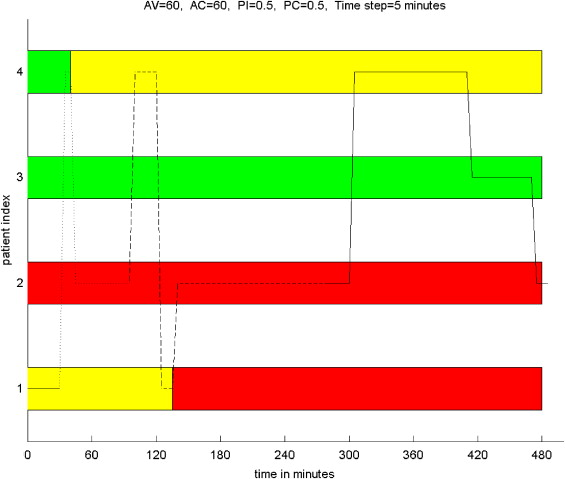
\includegraphics[width=0.8\textwidth]{FIGS/Dagata_etal_patients_profiles.jpg}
\end{center}
\vfill
\tiny Patient–HCW contact diagram for four patients and one HCW during one shift. Patient status: uninfected (green), infected with the non-resistant strain (yellow), infected with the resistant strain (red). HCW status: uncontaminated (plain), contaminated with the non-resistant strain (dotted), contaminated with the resistant strain (dashed)
\end{frame}


\begin{frame}
\begin{center}
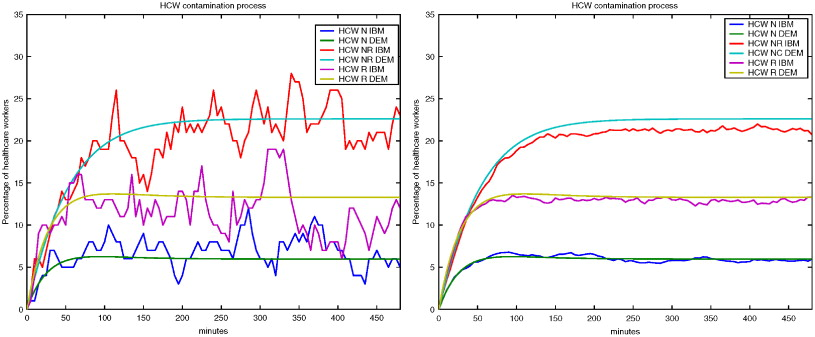
\includegraphics[width=\textwidth]{FIGS/Dagata_etal_comparisons.jpg}
\end{center}
\vfill
\tiny 
The left (respectively the right) figure corresponds to 1 trajectory (respectively the average over 80 trajectories) of the IBM during one shift, with no exit and admission of patients, and no changes in the infection status of patients
\end{frame}


\begin{frame}{Effectiveness of contact tracing in TB}
Tian, Osgood, Al-Azem \& Hoeppner. \href{https://doi-org.uml.idm.oclc.org/10.1177\%2F1090198113493910}{Evaluating the Effectiveness of Contact Tracing on Tuberculosis Outcomes in Saskatchewan Using Individual-Based Modeling}, Health Education \& Behavior (2013)
\end{frame}


\begin{frame}
\begin{center}
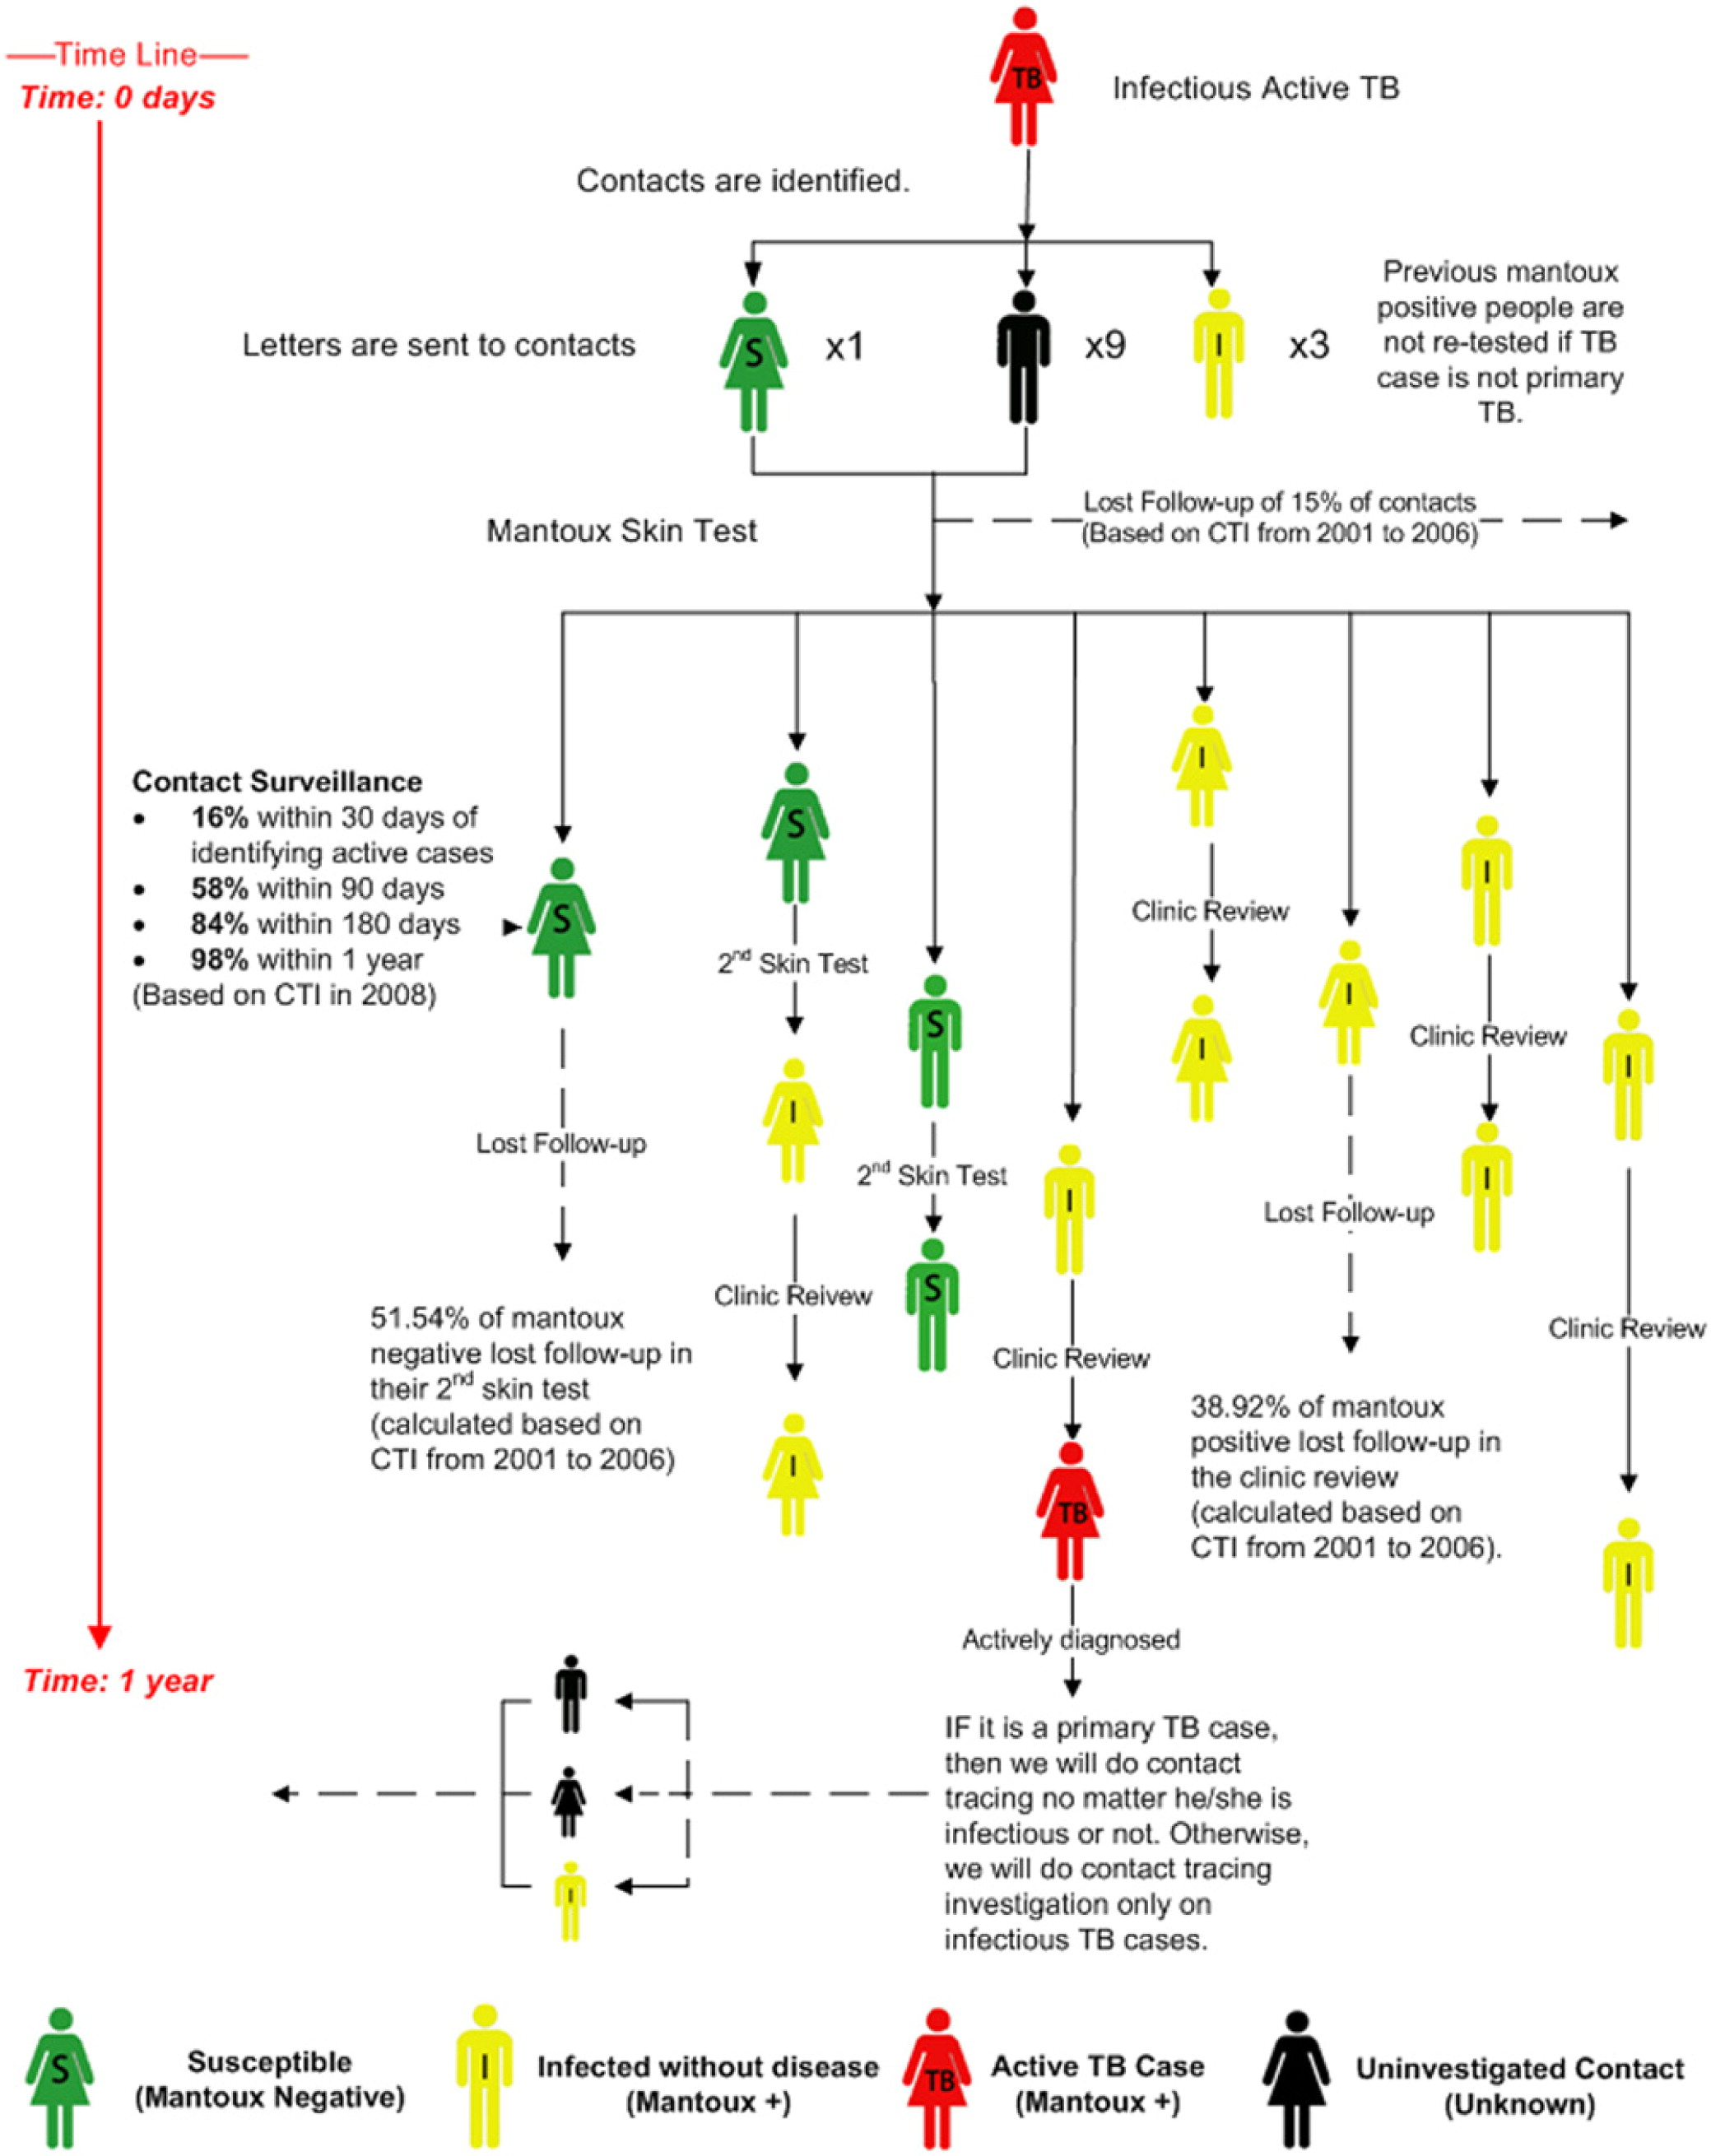
\includegraphics[width=\textwidth]{FIGS/TianOsgood_etal_TB_CT.jpeg}
\end{center}
\end{frame}

\begin{frame}
\begin{center}
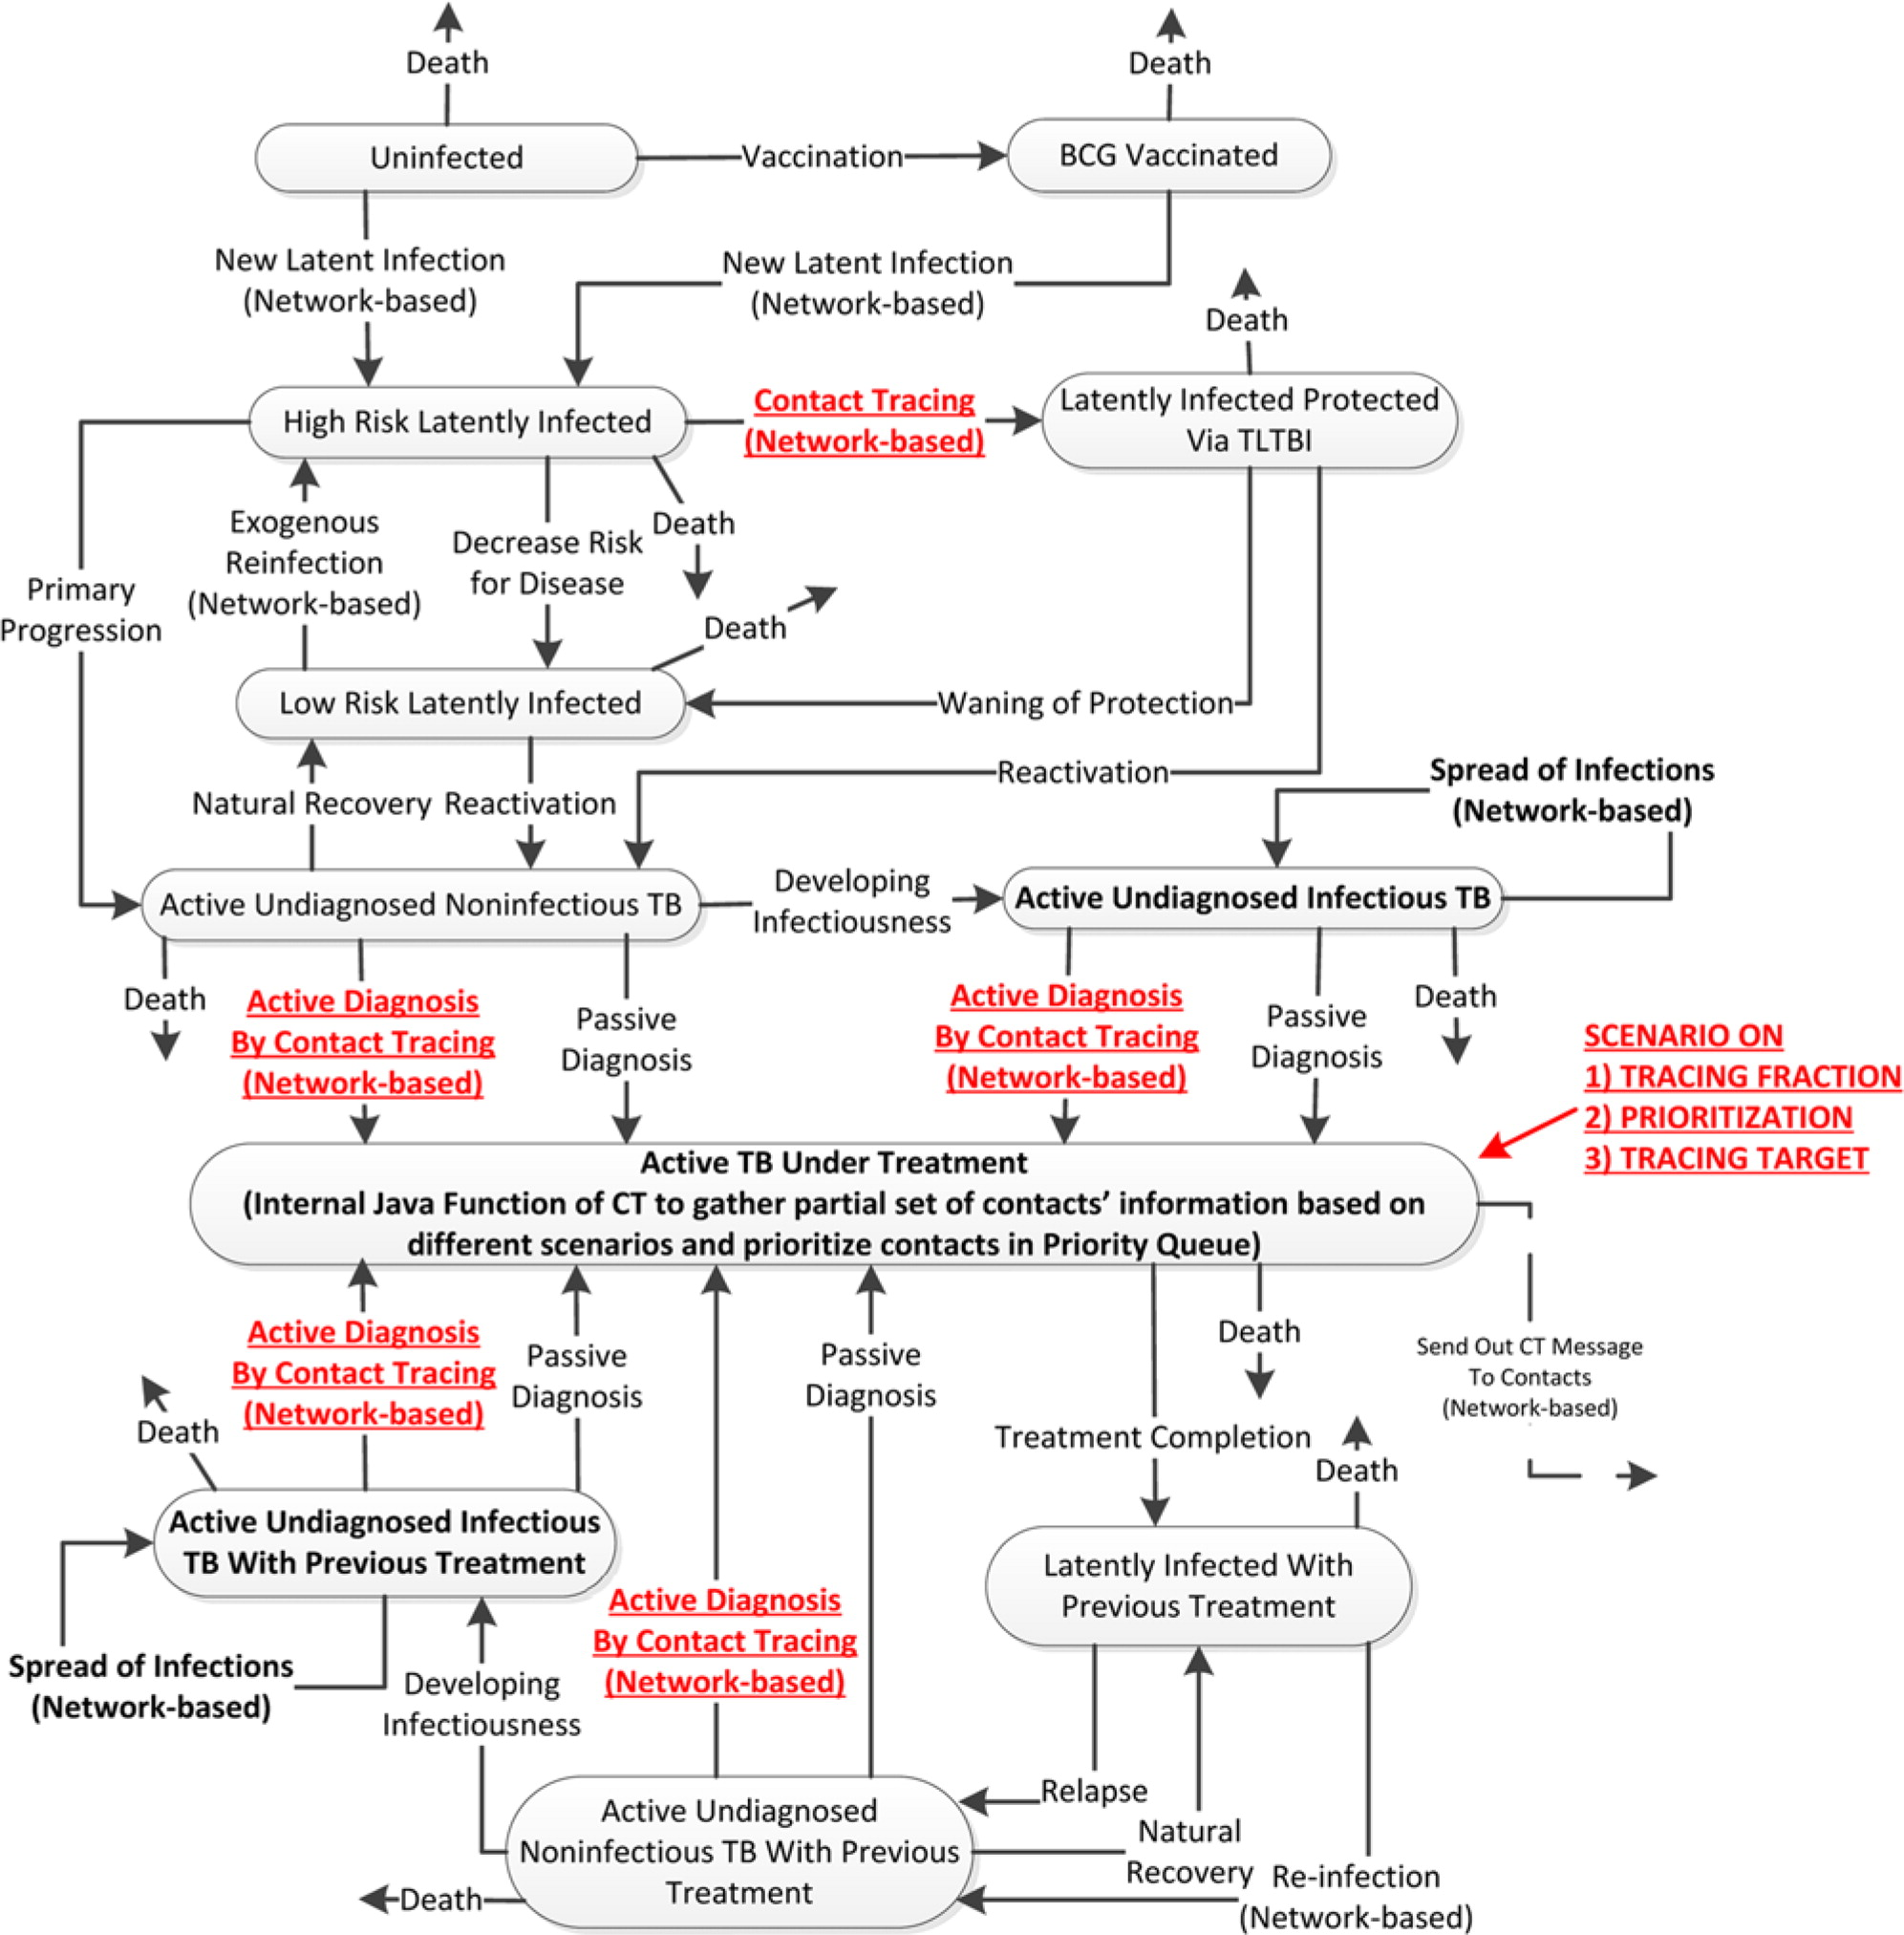
\includegraphics[width=\textwidth]{FIGS/TianOsgood_etal_state_flow_agent.jpeg}
\end{center}
\end{frame}


\begin{frame}
\begin{center}
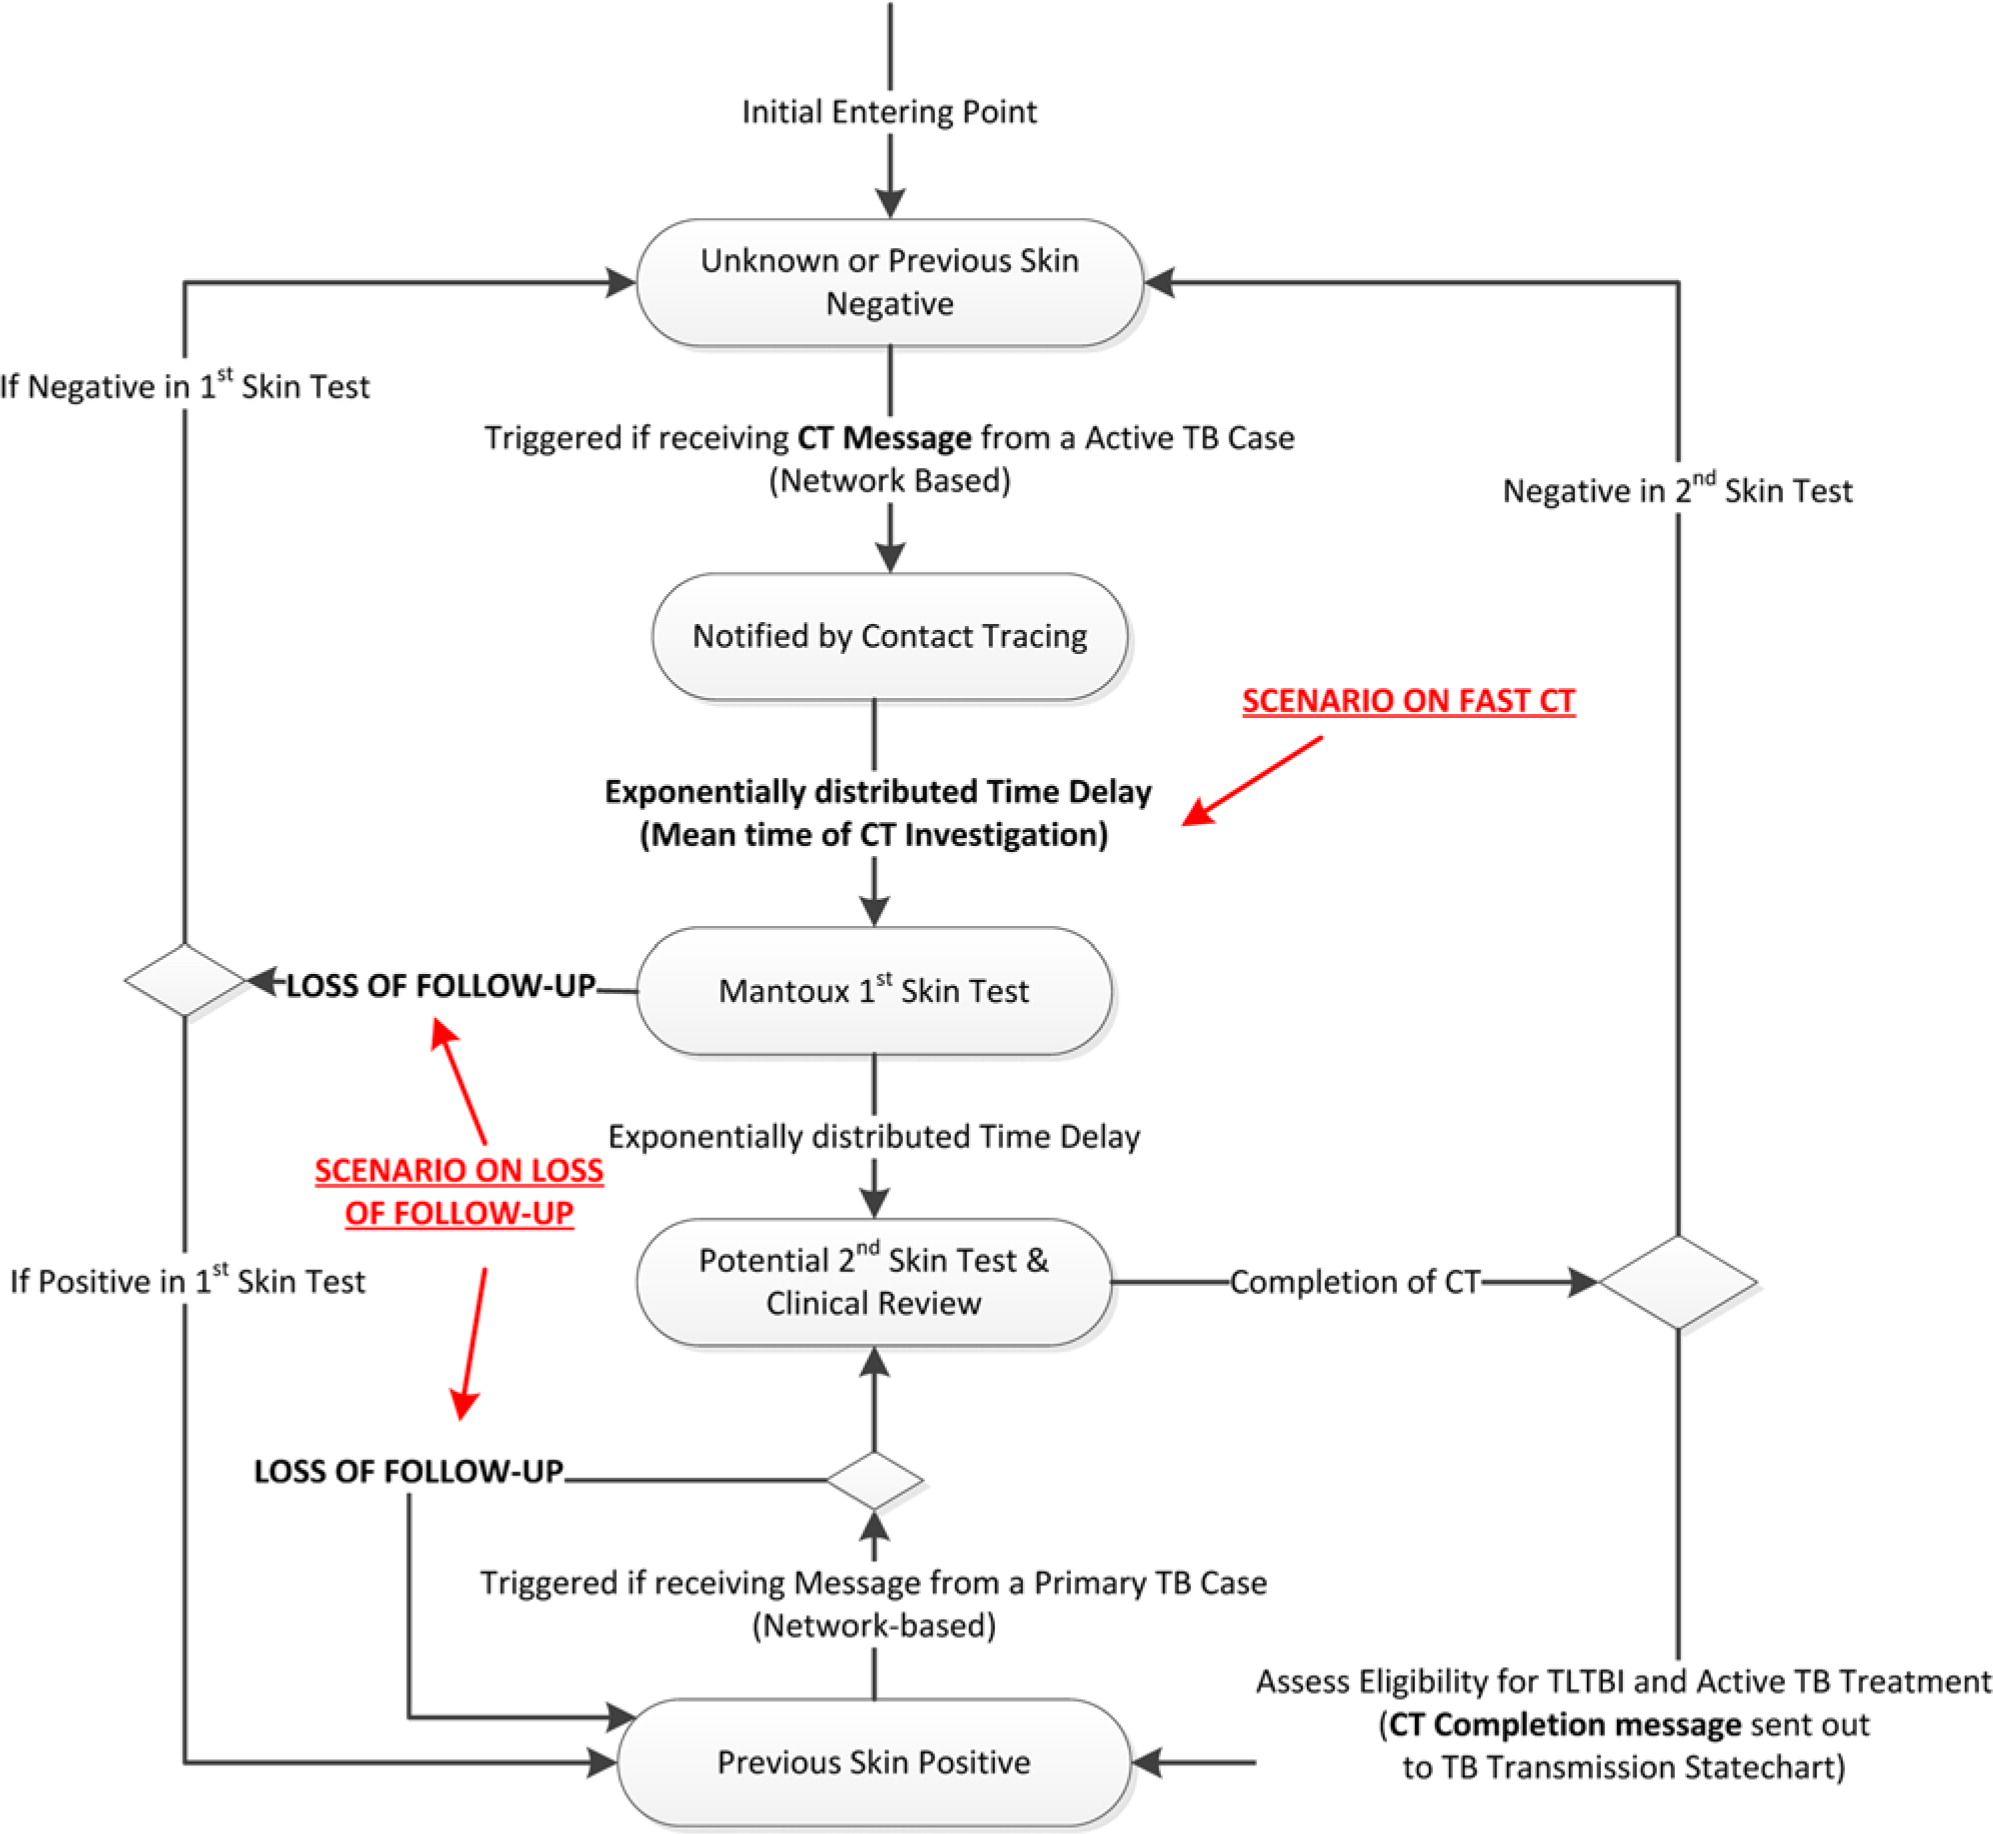
\includegraphics[width=\textwidth]{FIGS/TianOsgood_etal_model_CT.jpeg}
\end{center}
\end{frame}



\begin{frame}
They can then formulate scenarios
\begin{center}
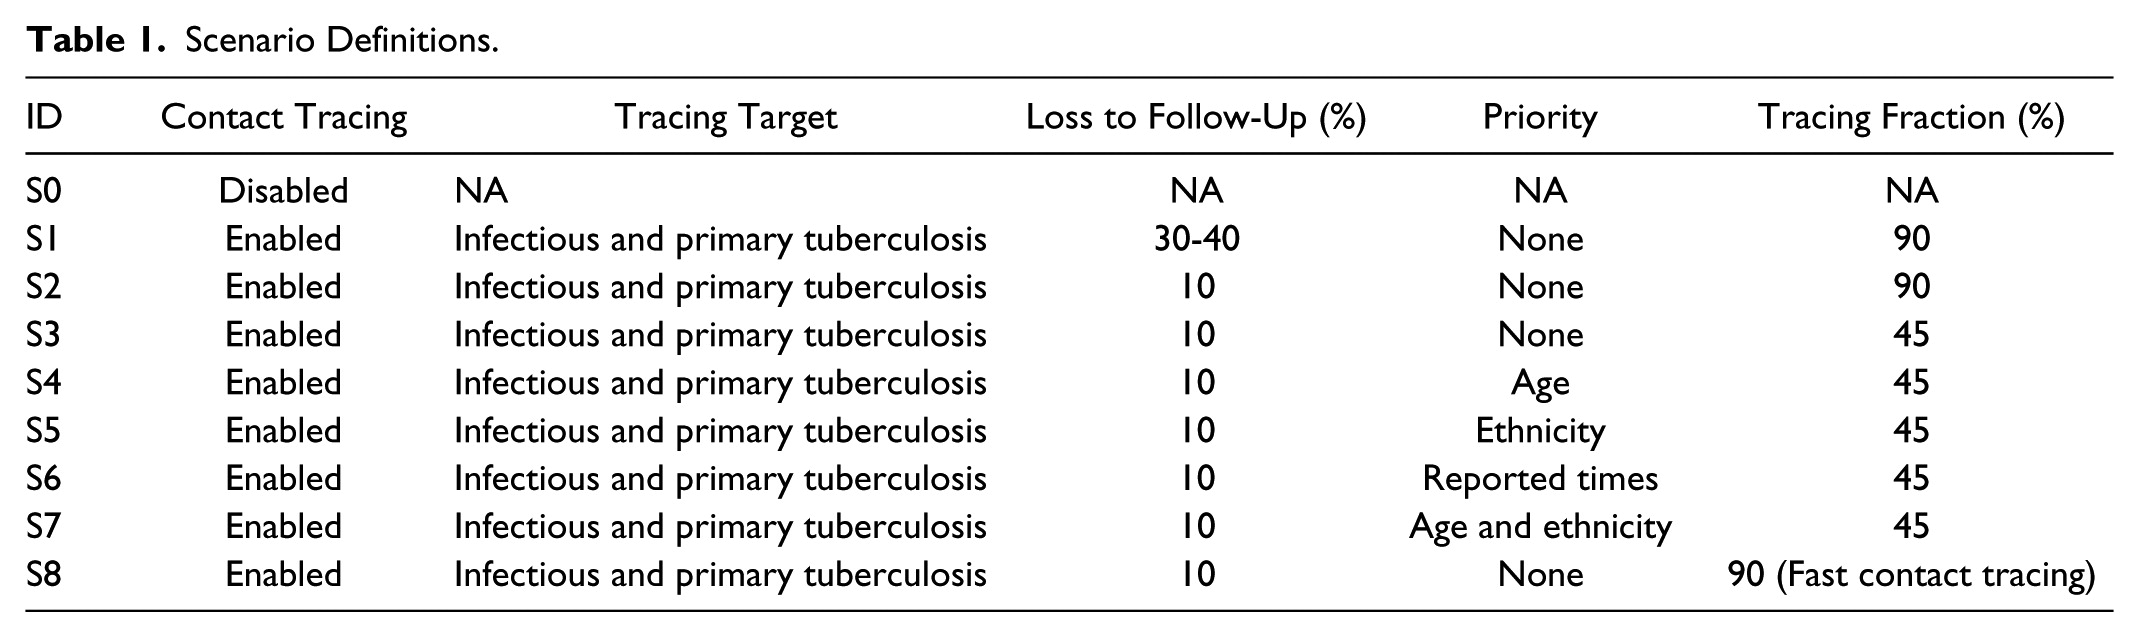
\includegraphics[width=\textwidth]{FIGS/TianOsgood_etal_scenarios.jpeg}
\end{center}
They then run these scenarios and compare results
\end{frame}


\begin{frame}
\begin{center}
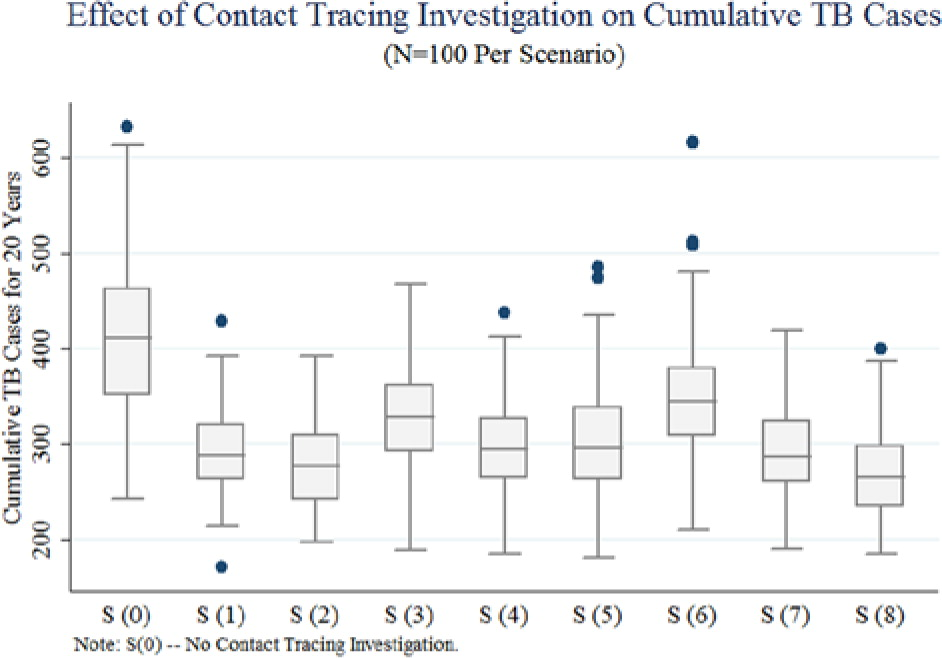
\includegraphics[width=\textwidth]{FIGS/TianOsgood_etal_scenario_results.jpeg}
\end{center}
\end{frame}


\begin{frame}{Contacts during Hajj}
Tofighi, Asgary, Tofighi, Najafabadi, Arino, Amiche, Rahman, McCarthy, Bragazzi, Thommes,  Coudeville, Grunnill, Bourouiba and Wu. \href{http://dx.doi.org/10.2139/ssrn.3678581}{Estimating Social Contacts in Mass Gatherings for Disease Outbreak Prevention and Management (Case of Hajj Pilgrimage)}, Tropical Diseases, Travel Medicine and Vaccines
\end{frame}

\begin{frame}{Contacts during Hajj}
In a mass gathering event like Hajj, lots of people come together originating from many countries
\vfill
So if propagation occurs during the event, this has the capacity to spread infection far and wide when individuals (pilgrims here) return home
\vfill
Contacts during part of the event are really specific in their configuration
\end{frame}


\begin{frame}{The setup}
Word of warning: I am quite fuzzy on the specifics :)
\vfill
Pilgrims enter Masjid al-Haram mosque through several gates
\vfill
Proceed to Mataaf (area around Kaaba), circle the Kaaba 7 times counterclockwise (process is the \emph{Tawaf})
\vfill
Then do seven trips between Safa and Marwah (process is the \emph{Sa'ee})
\end{frame}


% \begin{frame}
% 
% ![bg contain](https://upload.wikimedia.org/wikipedia/commons/thumb/7/7e/Great_Mosque_of_Mecca.jpg/1280px-Great_Mosque_of_Mecca.jpg)
% 
% \end{frame} 

\begin{frame}
As you can gather from this:
\begin{itemize}
\item Typically high density crowds
\item Very specific mixing patterns
\end{itemize}
\vfill
Opportunities for transmission are very high
\vfill
However, control mechanisms are also available
\vfill
$\implies$ understanding contact patterns and frequency would help
\end{frame}


\begin{frame}
\begin{center}
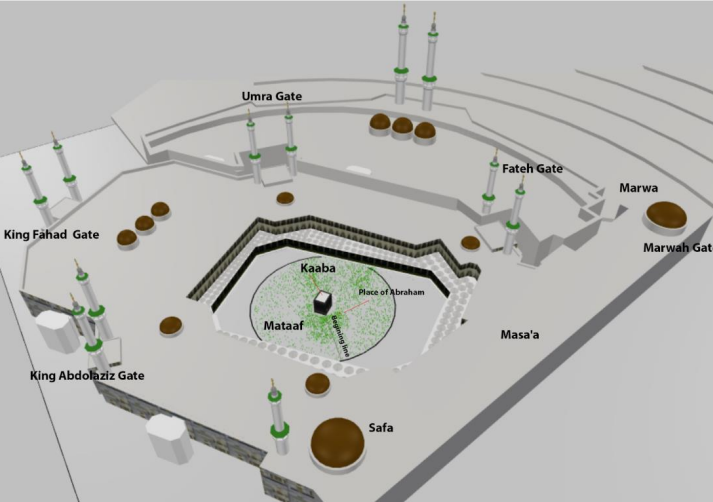
\includegraphics[width=\textwidth]{FIGS/ABM_Hajj_MAH_3Dmodel.png}
\end{center}
\end{frame}


\begin{frame}
\begin{center}
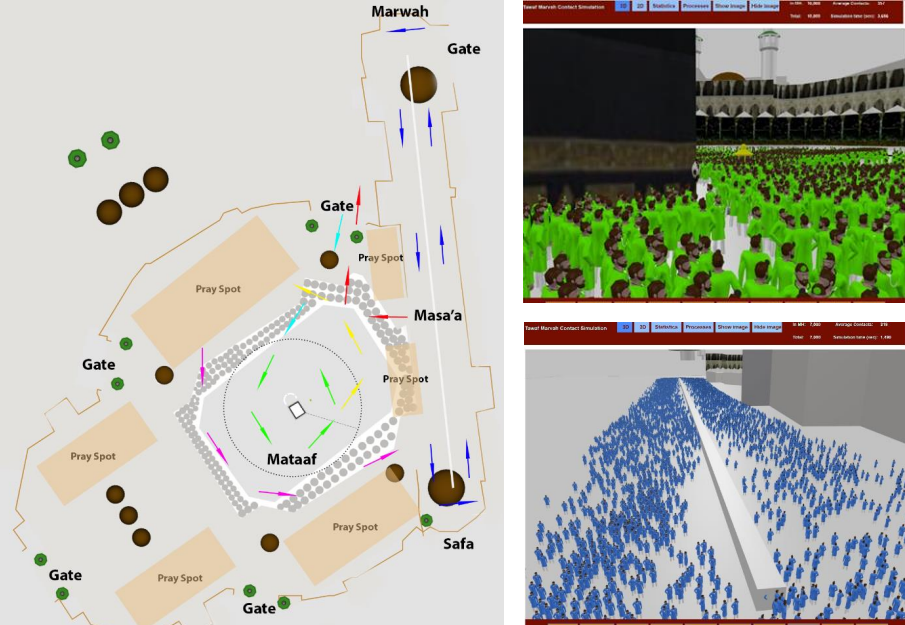
\includegraphics[width=\textwidth]{FIGS/ABM_Hajj_setup.png}
\end{center}
\end{frame}


\begin{frame}
\begin{center}
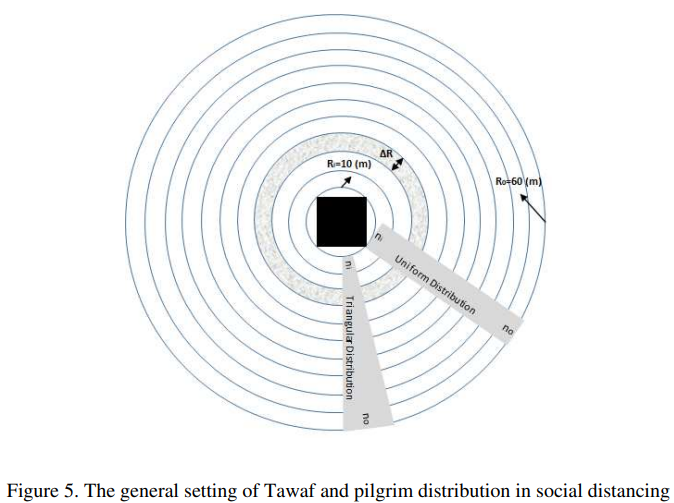
\includegraphics[width=\textwidth]{FIGS/ABM_Hajj_config_tawaf.png}
\end{center}
\end{frame}


%%%%%%%%%%%%%%%%%%%%%%%%%%%%%
%%%%%%%%%%%%%%%%%%%%%%%%%%%%%
%%%%%%%%%%%%%%%%%%%%%%%%%%%%%
%%%%%%%%%%%%%%%%%%%%%%%%%%%%%
\section{Network models}
%%%%%%%%%%%%%%%%%%%%%%%%%%%%%
%%%%%%%%%%%%%%%%%%%%%%%%%%%%%
\subsection{Why use network models}

\begin{frame}{Understand contact processes}
Classic models allow a certain degree of flexibility, for instance by using specific incidence functions or group models, but this remains limited and an approximation
\vfill
Like ABM, network models are used to make more realistic descriptions of the transmission of pathogens
\end{frame}


\begin{frame}{Human life is organised in networks}
Family
\vfill
Friends
\vfill
Workplace
\vfill
$\ldots$
\vfill
Social network theory has been used for years, e.g., in a professional context (e.g., how to fluidify interactions within a company)
\end{frame}

% \subsection{Les réseaux sociaux}
% 
% \begin{frame}
% 
% - Avant de considérer des épidémies dans des réseaux, quelques notions de réseaux sociaux, parce que c'est utile de façon générale pour comprendre les réseaux
% - Les méthodes en réseaux sociaux introduisent des mesures qui permettent d'évaluer certaines propriétés des graphes et qui sont utiles à connaître
% - Un réseau est un graphe (mathématique), orienté ou non, dans lequel les arcs représentent les connections (quelles qu'elles soient) entre les individus, qui sont les nœuds du graphe
% 
% \end{frame} 
% 
% 
% 
% \begin{frame}
% 
%  Contexte
% 
% - $\mathcal{G}(\mathcal{V},\mathcal{E})$ un graphe non orienté
% - $\mathcal{D}(\mathcal{V},\mathcal{A})$ un digraphe (graphe orienté)
% - $\mathcal{V}$ l'ensemble des nœuds (*vertices* en anglais)
% - $\mathcal{E}$ l'ensemble des arcs dans le cas non orienté (*edges* en anglais)
% - $\mathcal{A}$ l'ensemble des arcs dans le graphe orienté (*arcs* en anglais)
% 
% \end{frame} 
% 
% 
% \begin{frame}
% 
%  Exemple du réseau de transport aérien
% 
% - Je vais illustrer avec des données du réseau de transport aérien mondial
% - Données assez bonnes (très bonnes parfois), et un avantage flagrant:
%   - Quand un avion part de quelque part et arrive ailleurs, c'est quelque chose d'assez .. déterministe
% 
% \end{frame} 
% 
% 
% \begin{frame}
% 
% ![bg contain](https://raw.githubusercontent.com/julien-arino/petit-cours-epidemio-mathematique/main/FIGS/world_graph-degree.png)
% 
% 
% \end{frame} 
% 
% 
% \begin{frame}
% 
% ![bg contain](https://raw.githubusercontent.com/julien-arino/petit-cours-epidemio-mathematique/main/FIGS/Manitoba_network_schema_planar_oriented.png)
% 
% 
% \end{frame} \begin{frame}
% 
%  Densité du graphe
% 
% Un graph (resp. digraphe) est **complet** si toute paire de nœuds est connecté (resp. est connecté par un arc dans chaque direction)
% 
% S'il y a $n=|\mathcal{V}|$ nœeuds dans le graphe, alors il y a $n(n-1)/2$ (resp. $n(n-1)$) arcs dans le graphe (resp. digraphe) complet
% 
% (On ne compte pas les connections d'un nœud sur lui même)
% 
% Densité de $\mathcal{G}$ (graphe non orienté)
% $$
% \mathsf{dens}_\mathcal{G}=\frac{2\ |\mathcal{E}|}{n(n-1)}
% $$
% Densité de $\mathcal{D}$ (graphe orienté)
% $$
% \mathsf{dens}_\mathcal{D}=\frac{|\mathcal{A}|}{n(n-1)}
% $$
% 
% \end{frame} \begin{frame}
% 
%  Densité des digraphes considérés
% 
% | Digraphe |  nœuds |  arcs | densité |
% |\end{frame} \begin{frame}\end{frame} \begin{frame}\end{frame} \begin{frame}-|:\end{frame} \begin{frame}\end{frame} \begin{frame}-:|:\end{frame} \begin{frame}\end{frame} \begin{frame}:|:\end{frame} \begin{frame}\end{frame} \begin{frame}-:|
% | Manitoba | 24 | 64 | 0.1159 |
% | Canada | 222 | 804 | 0.0164 |
% | Amérique du Nord | 934 | 7,814 | 0.009 |
% | Global | 3403 | 32,576 | 0.0028 |
% 
% \end{frame} \begin{frame}
% 
%  Degré
% 
% **Degré** $d_\mathcal{G}(v)$ du nœud $v\in\mathcal{V}$ dans $\mathcal{G}$: nombre d'arcs incidents à $v$
% 
% **Degré entrant** $d^-_\mathcal{D}(v)$ du nœud $v\in\mathcal{V}$ dans $\mathcal{D}$: nombre d'arcs avec tête $v$
% 
% **Degré sortant** $d^+_\mathcal{D}(v)$ du nœud $v\in\mathcal{V}$ dans $\mathcal{D}$: nombre d'arcs avec queue $v$
% 
% **Degré** $d_\mathcal{D}(v)$ du nœud $v\in\mathcal{V}$ dans $\mathcal{D}(\mathcal{V},\mathcal{A})$: nombre d'arcs incidents à $v$ dans le graphe non orienté sous-jacent $\mathcal{G}$ de $\mathcal{D}$ (où tout arc est considérée comme un arc ``bidirectionnel'')
% 
% \end{frame} \begin{frame}
% 
%  Degré entrant global du réseau de transport aérien
% 
% | Ville | Pays | Degré entrant | Rang |
% |\end{frame} \begin{frame}\end{frame} \begin{frame}|\end{frame} \begin{frame}\end{frame} \begin{frame}\end{frame} \begin{frame}|:\end{frame} \begin{frame}\end{frame} \begin{frame}\end{frame} \begin{frame}-:|:\end{frame} \begin{frame}-:| 
% | Londres | GB | 365 | 1 |
% | Paris | France | 294 | 2 |
% | Frankfurt | Allemagne | 287 | 3 |
% | Atlanta | USA | 249 | 4 |
% | New York | USA | 241 | 5 |
% | Moscou | Russie | 225 | 6 |
% | Amsterdam | Pays-Bas | 204 | 7 |
% | Chicago | USA | 203 | 8 |
% | Munich | Allemagne | 200 | 9 |
% | Milan | Italie | 181 | 10 |
% 
% \end{frame} \begin{frame}
% 
%  Le degré change pendant l'année 
% 
% Les graphes sont dynamiques !
% 
% ![bg right:72%](https://raw.githubusercontent.com/julien-arino/petit-cours-epidemio-mathematique/main/FIGS/IATA_outdegree_YEA_2005_to_2010.png)
% 
% 
% \end{frame} \begin{frame}
% 
%  Plus court chemin
% 
% Soit $\mathcal{D}$ un digraphe. Le (ou les) plus court(s) chemin(s) de $i$ à $j$ dans $\mathcal{V}$:
% $$
% d_\mathcal{D}(i,j)=\min_{p\in\mathcal{P}(i,j)} f(p)
% $$
% où $\mathcal{P}(i,j)$ est l'ensemble des chemins de $i$ à $j$ et $f(p)$ est un valuation des arcs dans le chemin $p$. On définit $d_\mathcal{D}(i,j)=\infty$ s'il n'existe pas de chemin de $i$ à $j$ 
% 
% $f(p)$ peut être
% - le nombre d'arcs dans $p$ de $i$ à $j$ (**distance géodésique**)
% - Distance du grand cercle des arcs de $p$
% - durée des vols des arcs de $p$
% 
% \end{frame} \begin{frame}
% 
%  Excentricité
% 
% **Excentricité** (ou **nombre de Köonig**) du nœud $v\in\mathcal{V}$ dans $\mathcal{G}(\mathcal{V},\mathcal{E})$
% $$
% e(v)=\max_{v'\in\mathcal{V}}d_\mathcal{D}(v,v')
% $$
% **Excentricité entrante** du nœud $v\in\mathcal{V}$ dans $\mathcal{D}(\mathcal{V},\mathcal{A})$
% $$
% e^-(v)=\max_{v'\in\mathcal{V}}d_\mathcal{D}(v',v)
% $$
% **Excentricité sortante** du nœud $v\in\mathcal{V}$ dans $\mathcal{D}(\mathcal{V},\mathcal{A})$
% $$
% e^+(v)=\max_{v'\in\mathcal{V}}d_\mathcal{D}(v,v')
% $$
% 
% \end{frame} \begin{frame}
% 
% | Graphe | $e^-(YWG)$ | $e^+(YWG)$ |
% |\end{frame} \begin{frame}\end{frame} \begin{frame}--|\end{frame} \begin{frame}\end{frame} \begin{frame}\end{frame} \begin{frame}\end{frame} \begin{frame}|\end{frame} \begin{frame}\end{frame} \begin{frame}\end{frame} \begin{frame}\end{frame} \begin{frame}|
% | Manitoba | 2 | 3 (Lynn Lake) |
% | Canada | 7 $^{(*)}$ | 7 $^{(*)}$ |
% | Amérique du Nord | 7 $^{(**)}$| 8 (Stony River) |
% | Global | 7 $^{(***)}$ | 8 (Stony River) |
% 
% | <!-- --> | <!-- --> |
% |\end{frame} \begin{frame}|\end{frame} \begin{frame}|
% | ( * ) | Peawanuck (ON), Port Hope Simpson (NL) |
% ( ** ) | ( * ) + Lopez Island, Kwethluk, Chuathbaluk |
% ( *** ) | ( ** ) + Hooker Creek, Birdsville, Beni, Balalae, Thargomindah |
% 
% \end{frame} \begin{frame}
% 
%  Rayon
% 
% **Rayon** de $\mathcal{G}$
% $$
% \rho_\mathcal{G}=\min_{v\in\mathcal{V}}e(v)
% $$
% **Rayon entrant** de $\mathcal{D}$
% $$
% \rho_\mathcal{D}^-=\min_{v\in\mathcal{V}}e^-(v)
% $$
% **Rayon sortant** de $\mathcal{D}$
% $$
% \rho_\mathcal{D}^+=\min_{v\in\mathcal{V}}e^+(v)
% $$
% 
% rayon = $\min(\max(\cdot))$ $\rightarrow$ directionalité
% 
% \end{frame} \begin{frame}
% 
%  Rayon du réseau de transport aérien
% 
% | Graphe | $\rho^-$ | $\rho^+$ |
% |\end{frame} \begin{frame}\end{frame} \begin{frame}--|\end{frame} \begin{frame}\end{frame} \begin{frame}\end{frame} \begin{frame}-|\end{frame} \begin{frame}\end{frame} \begin{frame}\end{frame} \begin{frame}-|
% | Manitoba | 2 | 3 |
% | Canada | 6 | 6 |
% | Amérique du Nord | 6 | 7 |
% | Global | 7 | 7 |
% 
% 
% \end{frame} \begin{frame}
% 
%  Centre d'un graphe
% 
% **Centre** de $\mathcal{D}$:
% $$
% \mathcal{C}_\mathcal{D}=\left\{v\in\mathcal{V}:e(v)=\rho_\mathcal{D}\right\}
% $$
% 
% \end{frame} \begin{frame}
% 
%  Centre du réseau de transport aérien
% 
% | Graphe | $\mathcal{C}^-$ | $\\\|\mathcal{C}^-\\\|$ | $\mathcal{C}^+$ | $\\\|\mathcal{C}^+\\\|$ |
% |\end{frame} \begin{frame}|\end{frame} \begin{frame}|\end{frame} \begin{frame}|\end{frame} \begin{frame}|\end{frame} \begin{frame}|
% | Manitoba | 2 | 1 (YWG) | 3 | 7 |
% | Canada | 6 | 1 (YTO) | 6 | 1 (YTO) |
% | Amérique du Nord | 6 | 1 (YTO) | 7 | 18 |
% | Global | 7 | 131 | 7 | 20 |
% 
% $\{$YYC,YEA,Halifax,Kelowna,Moncton,YMQ,YOW,Quebec,St John's,YTO,YVR, Victoria,YWG$\}\subset\mathcal{C}^-$
% 
% $\{$Toronto,Vancouver$\}\subset\mathcal{C}^+$
% 
% \end{frame} \begin{frame}
% 
%  Diamètre
% 
% **Diamètre** de $\mathcal{D}$
% $$
% \mathsf{diam}_\mathcal{D}=\max_{v\in\mathcal{V}}e(v)
% $$
% 
% diamètre = max(max(.)) $\rightarrow$ pas de directionalité
% 
% \end{frame} \begin{frame}
% 
% 
% Graphe | Diamètre |
% |\end{frame} \begin{frame}\end{frame} \begin{frame}|:\end{frame} \begin{frame}\end{frame} \begin{frame}--:|
% | Manitoba | 5 |
% | Canada | 12 |
% | Amérique du Nord | 13 |
% | Global | 13 |
% 
% 
% \end{frame} \begin{frame}
% 
%  Péripherie d'un graphe
% 
% **Péripherie** de $\mathcal{D}$ 
% $$
% \mathcal{P}_\mathcal{D}=\left\{v\in\mathcal{V}:e(v)=\mathsf{diam}_\mathcal{D}\right\}
% $$
% 
% \end{frame} \begin{frame}
% 
% | Graphe | Péripherie entrante | Péripherie sortante |
% |\end{frame} \begin{frame}\end{frame} \begin{frame}--|\end{frame} \begin{frame}\end{frame} \begin{frame}\end{frame} \begin{frame}\end{frame} \begin{frame}\end{frame} \begin{frame}\end{frame} \begin{frame}\end{frame} \begin{frame}|\end{frame} \begin{frame}\end{frame} \begin{frame}\end{frame} \begin{frame}\end{frame} \begin{frame}\end{frame} \begin{frame}\end{frame} \begin{frame}\end{frame} \begin{frame}|
% | Manitoba | Lynn Lake | Cross Lake, Red Sucker Lake, Brandon |
% | Canada | Peawanuck | Peawanuck, Port Hope Simpson | Port Hope Simpson |
% | Amérique du Nord | Stony River | Peawanuck, Port Hope Simpson |
% | Global | Stony River, Hooker Creek, Peawanuck | Hooker Creek, Beni, Peawanuck, Port Hope Simpson |
% 
% \end{frame} \begin{frame}
% 
%  Bien d'autres mesures
% 
% - betweenness
% - closeness
% - $k$-cores
% - $\ldots$
% 
% \end{frame} \begin{frame}
% 

\subsection{Cadre général des modèles en réseaux}

% 
% \end{frame} \begin{frame}
% 
% - Voir par exemple 
%   - Newman. [Spread of epidemic disease on networks](https://doi.org/10.1103/PhysRevE.66.016128), 2002
%   - Keeling & Eames. [Networks and epidemic models](https://doi.org/10.1098/rsif.2005.0051), 2005
%   - Meyers, Pourbohloul, Newman, Skowronski & Brunham. [Network theory and SARS: predicting outbreak diversity](https://doi.org/10.1016/j.jtbi.2004.07.026), 2005
%   - Meyers, Newman & Pourohloul. [Predicting epidemics on directed contact networks](https://doi.org/10.1016/j.jtbi.2005.10.004), 2006
%   - Bansal, Read, Pourbohloul & Meyers. [The dynamic nature of contact networks in infectious disease epidemiology](https://doi.org/10.1080/17513758.2010.503376), 2010 
% 
% 
% \end{frame} \begin{frame}
% 
% - Typiquement, on considère un graphe (ou digraphe selon les cas) dans lequel:
%   - chaque nœud est un individu 
%   - l'existence d'un arc de $i$ vers $j$ indique que $i$ est en contact avec $j$ et peut lui transmettre l'infection
%   - dans le cas non orienté, l'existence d'un arc de $i$ vers $j$ implique celle d'un arc (le même) de $j$ vers $i$ et établit que les deux individus sont connectés
% - La connexion n'est pas permanente, mais décrit plutôt la possibilité d'une connexion: $i$ et $j$ entrent en contact de façon régulière
% 
% \end{frame} \begin{frame}
% 
%  Matrice d'adjacence
% 
% On utilisera souvent la **matrice d'adjacence** $A=[a_{ij}]$, dans laquelle $a_{ij}=1$ si le nœud $i$ a un lien vers le nœud $j$ et $a_{ij}=0$ sinon
% 
% On écrit parfois $A(\mathcal{D})$ pour indiquer que $A$ est la matrice d'adjacence du digraphe $\mathcal{D}$, et dans l'autre sens, $\mathcal{D}(A)$ pour indiquer que le graphe est construit en utilisant la matrice d'adjacence
% 
% Si le graphe est non orienté, alors $A$ est symmétrique
% 
% \end{frame} \begin{frame}
% 
%  Nature du réseau
% 
% - Parfois on dispose de données précises sur les liens entre individus (sondages, etc.)
% - Souvent on idéalise des réseaux, on choisit des réseaux avec des propriétés données
% 
% \end{frame} \begin{frame}
% 
%  La distribution des degrés du (di)graphe
% 
% La **transmissibilité** $T$ d'une maladie dans un graphe est la probabilité moyenne qu'un individu infectieux transmette la maladie à un individu susceptible avec qui il/elle est en contact
% 
% Dans un réseau non corrélé,
% $$
% T_c = \frac{\langle k\rangle}{\langle k^2\rangle-\langle k\rangle}
% $$
% où $\langle k\rangle$ et $\langle k^2\rangle$ sont le degré moyen et la moyenne du carré du degré
% 
% Il est nécessaire que $T>T_c$ pour qu'un *outbreak* devienne une épidémie majeure
% 
% \end{frame} \begin{frame}
% 
\begin{frame}{La librairie EpiModel}
Jenness SM, Goodreau SM and Morris M. \href{https://doi.org/10.18637\%2Fjss.v084.i08}{EpiModel: An R Package for Mathematical Modeling of Infectious Disease over Networks}. Journal of Statistical Software. 2018; 84(8): 1-47
\end{frame} 


\begin{frame}{EpiModel}
\code{R} library providing tools to simulate and analyse network epidemiological models
\vfill
Provides two types of approaches
\begin{itemize}
\item Simulation of ODE compartmental models (not so interesting)
\item Simulation of network models
\end{itemize}
\vfill
Their \href{https://www.epimodel.org}{website} has several useful tutorials
\vfill
Part of the \href{http://statnet.org/}{statnet} meta-library
\end{frame}

\end{document}
